\documentclass{cake-classes/short-report-fa}
\usepackage{booktabs}
\begin{document}
\درج‌عنوان‌سند

\قسمت{مقدمه}
در این متن، معماری پیشنهادی برای نسخهٔ اول پلتفرم ابری پروژه کیک روباتیک معرفی شده است.

\قسمت{معماری}

معماری انتخاب شده در شکل \رجوع{معماری} آمده است. بلوک‌های این شکل هر کدام یک سرویس هستند که از یک یا چند میکروسرویس تشکیل می‌شوند. خط سفید به معنای ارتباط دوطرفه و پیکان به معنای جریان داده یک‌طرفه می‌باشد. سرویس‌های زرد رنگ در داخل تیم توسعه داده نمی‌شوند.

همچنین، لازم به ذکر است که در این شکل تنها اتصالات کلیدی ذکر شده است؛ برای مثال، سرویس احراز هویت و دسترسی (\مل{Auth})، تقریبا با تمام سرویس‌های بک‌اند ارتباط دارد که در شکل نیامده است.

در سمت راست نمودار هم سرویس‌های رباتیک ابری دیده می‌شود که هنوز تصمیم‌گیری برای آن‌ها کامل نشده است.

\begin{figure}[p]
	\centering
	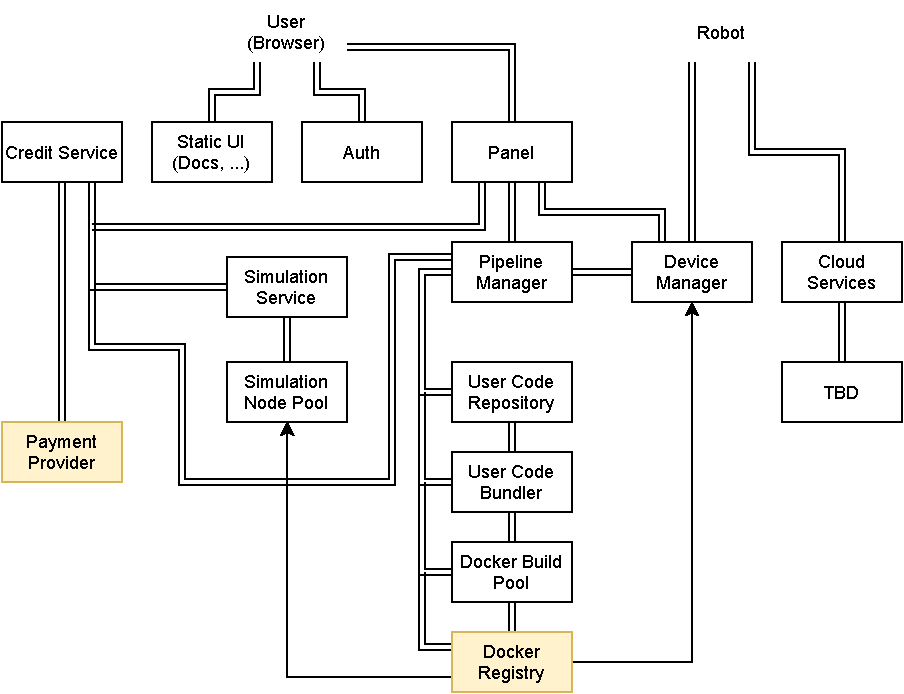
\includegraphics[width=\linewidth]{arch.pdf}
	\شرح{معماری انتخاب شده}
	\برچسب{معماری}
\end{figure}
\end{document}
